\documentclass[twoside]{amsart}
\usepackage{amssymb,latexsym}
\usepackage{amsfonts}
\usepackage{xspace}
\usepackage{enumerate}
\usepackage{graphics}
\usepackage{fitch}
\newcommand{\Rationals}{\mathbb{Q}{}}
\newcommand{\Reals}{\ensuremath{\mathbb{R}}\xspace}
\newcommand{\Integers}{\ensuremath{\mathbb{Z}{}}\xspace}
\newcommand{\solution}{\textsc{Solution}\xspace}
\newcommand{\problem}{\textsc{Problem}\xspace}
\newcommand{\Blank}{\mathrel{\phantom{=}}}
\newcommand{\ltrue}{\top}
\newcommand{\lfalse}{\bot}
\newcommand{\fOfg}{\ensuremath{f \circ g}\xspace}
\newcommand{\gOff}{\ensuremath{g \circ f}\xspace}
\newcommand{\eps}{\ensuremath{\epsilon}\xspace}
\newcommand{\iso}{\cong}
\newcommand{\niso}{\ncong}
\newcommand{\blank}{\vspace{5pt}}
\newcommand{\ind}{\hspace{.35in}}
\newcommand{\degree}{\ensuremath{^\circ}}
\newcommand{\real}{\mathop{\mathrm{real}}}
\newcommand{\img}{\mathop{\mathrm{img}}}
\newcommand{\first}{\mathop{\mathrm{first}}}
\newcommand{\second}{\mathop{\mathrm{second}}}
\begin{document}
\title{Answers to Chapter 9 Exercises - A Book of Abstract Algebra}
\author{Michael Welch}
\date{\today}
\maketitle

This document contains selected answers to exercises from chapter 9
of A Book of Abstract Algebra.


\begin{enumerate}[A.]
   \item \textsc{Isomorphism Is an Equivalence Relation among Groups}
	The following three facts about isomorphism are true for all groups:

	\blank
	\begin{enumerate}[(i)]
	   \item Every group is isomorphic to itself.
		\item If $G_1 \iso G_2$, then $G_2 \iso G_1$.
		\item If $G_1 \iso G_2$ and $G_2 \iso G_3$, then $G_1 \iso G_3$.
	\end{enumerate}
	\blank

	Fact (i) asserts that for any group $G$, there exists an isomorphism 
	from $G$ to $G$.

	Fact (ii) asserts that, if there is an isomorphism $f$ from $G_1$ to
	$G_2$, there must be some isomorphism from $G_2$ to $G_1$. Well, the
	inverse of $f$ is such an isomorphism.

	Fact (iii) asserts that, if there are isomorphisms $f : G_1 \to G_2$ and
	$g : G_2 \to G_3$, there must be an isomorphism from $G_1$ to $G_3$. One can
	easily guess that $g \circ f$ is such an isomorphism. The details of
	(i), (ii), and (iii) are left as exercises.
	\blank

   \begin{enumerate}[1]
	
	\item Let $G$ be any group. If $\epsilon : G \to G$ is the identity
	function, $\epsilon(x) = x$, show that $\epsilon$ is an isomorphism.

	\blank \noindent \solution To show this, we must show that
	$\epsilon$ is a bijective function and that the property
	$\epsilon(ab)=\epsilon(a)\epsilon(b)$.

	It is injective because if $\epsilon(a)=\epsilon(b)$ then we know
	$a=b$. It is surjective because for any $y$ I know $x = [\epsilon(y)]^{-1}$
	for $x=y$. Therefore it is bijective.

	The isomorphic property is trivial to show. 
	\begin{align*}
	    \epsilon(ab) &= ab && \text{Definition of identity} \\
		              &= \epsilon(a)\epsilon(b) && \text{Defn of identity twice}
	\end{align*}

	\item Let $G_1$ and $G_2$ be groups, and $f: G_1 \to G_2$ an isomorphism.
	Show that $f^{-1} : G_2 \to G_1$ is an isomorphism. [\textsc{Hint}:
	Review the discussion of inverse functions at the end of Chapter 6. Then,
	for arbitrary elements $c, d \in G_2$, there exist $a, b \in G_1$ such
	that $c = f(a)$ and $d = f(b)$. Note that $a = f^{-1}(c)$ and 
	$b = f^{-1}(d)$. Show that $f^{-1}(cd)=f^{-1}(c)f^{-1}(d)$.]

   \blank \noindent \solution Since $f$ is bijective we know that
	$f^{-1}$ is bijective. We know that $f(ab)=f(a)f(b)=cd$. Therefore
	$f^{-1}(cd)=ab=f^{-1}(c)f^{-1}(d)$. Therefore $f^{-1}$ is an isomorphism.

	\item Let $G_1$, $G_2$, and $G_3$ be groups, and let $f: G_1 \to G_2$ and
	$g:G_2 \to G_3$ be isomorphisms. Prove that $g \circ f : G_1 \to G_3$ is
	an isomorphism.

	\blank \noindent \solution The function $g \circ f$ is injective:
	Assume $(g \circ f)(a) = (g \circ f)(b)$. Then $g(f(a)) = g(f(b))$. But
	since $g$ is bijective we know that $f(a)=f(b)$. And since $f$ is
	bijective we know that $a=b$. Therefore $g \circ f$ is injective.

	\ind The function $g \circ f$ is surjective. Choose some element $y \in G_3$.
	Since $g$ is surjective we know there exist some $x \in G_2$ with
	the value $x = g^{-1}(y)$. Likewise, because $f$ is surjective
	we know there is some $z \in G_1$ with the value $z = f^{-1}(x)$. 
	Therefore $g \circ f$ is surjective and therefore it is bijective.

	Now we must show that $(g \circ f)(ab) = (g\circ f)(a)(g\circ f)(b)$.
	\begin{align}
		(g \circ f)(ab) &= g(f(ab))   \\
		                &= g(f(a)f(b))  && \text{$f$ is isomorphic (1)} \\
							 &= g(f(a)) g(f(b)) && \text{$g$ is isomorphic (2)} \\
							 &= (g \circ f)(a) (g\circ f)(b)
	\end{align}

   \end{enumerate}

	\item \textsc{Elements Which Correspond under an Isomophism}
	Recall that an isomorphism $f$ from $G_1$ to $G_2$ is a one-to-one
	correspondence between $G_1$ and $G_2$ satisfying $f(ab)=f(a)f(b)$.
	$f$ matches every element of $G_1$ with a corresponding element of
	$G_2$. It is important to note that:
	\blank

	\begin{enumerate}[(i)]
		\item $f$ matches the neutral element of $G_1$ with the neutral
		element of $G_2$.

		\item If $f$ matches an element $x$ in $G_1$ with $y$ in $G_2$,
		then, necessarily, $f$ matches $x^{-1}$ with $y^{-1}$.
		That is, if $x \leftrightarrow y$, then $x^{-1} \leftrightarrow
		y^{-1}$.

		\item $f$ matches a generator of $G_1$ with a generator of $G_2$.

      \blank
      \begin{center}
		\scalebox{1.2}{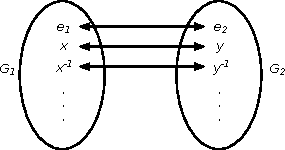
\includegraphics{img/chap9b.pdf}}
		\end{center}
		\blank

		The details of these statements are now left as an exercise. Let 
		$G_1$ and $G_2$ be groups, and let $f : G_1 \to G_2$ be an 
		isomorphism.

		\begin{enumerate}[1.]
			\item If $e_1$ deontes the neutral element of $G_1$ and $e_2$
			denotes the neutral element of $G_2$, prove that $f(e_1)=e_2$.
			[\textsc{Hint}: In any group, there is exactly one neutral
			element; show that $f(e_1)$ is the neutral element of $G_2$.]

			\setcounter{equation}{0}
			\blank \noindent \solution 
			\begin{align}
			   f(ae_1) &= f(a)   && \text{Identity}\\
				f(ae_1) &= f(a)f(e_1) && \text{Isomorphism}\\
				f(a)    &= f(a)f(e_1) && \text{(1) and (2)}\\
				f(a)e_2 &= f(a)f(e_1) && \text{Identity of $e_2$}\\
				    e_2 &= f(e_1)     && \text{Cancellation}
			\end{align}

			\item Prove the for each element $a$ in $G_1$, $f(a^{-1})
			= [f(a)]^{-1}$. (\textsc{Hint}: You may use Theorem 2 of 
			Chapter 4.)

			\setcounter{equation}{0}
			\blank \noindent \solution 
			\begin{align}
				f(aa^{-1}) &= f(e)          && \text{Inverses} \\
				f(aa^{-1}) &= f(a)f(a^{-1}) && \text{Isomorphism} \\
				f(e)       &= f(a)f(a^{-1}) && \text{(2) and (3)} \\
				f(a^{-1})  &= [f(a)]^{-1}   && \text{Theorem 2 of Chap 4 (3)}
			\end{align}

			\item If $G_1$ is a cyclic group with generator $a$, prove
			that $G_2$ is also a cyclic group, with generator $f(a)$.

			\blank \noindent \solution Choose any element $y \in G_2$. 
			Let $x = f^{-1}(y)$. We know that $x = a^n$ for some value of $n$.
			If $n=0$ then we have $y = f(e_1) = e_2 = [f(a)]^0$.
			If $n>0$ then $y = f(a^n) = \underbrace{f(a)f(a)\cdots f(a)}_{n
			\text{ times}} = [f(a)]^n$. Finally, if $n<0$ then
			$y = f(a^n) = \underbrace{f(a^{-1})f(a^{-1})\cdots f(a^{-1})}_{-n
			\text{ times}} = [f(a^{-1})]^{-n}$. From part 2 we know that
			$f(a^{-1}) = [f(a)]^{-1}$. Therefore 
			$[f(a^{-1})]^{-n} = ([f(a)]^{-1})^{-n}$. For each value of
			$n$ we have shown how to generate $y$ from $f(a)$. And since,
			$y$ was an arbitrary element of $G_2$ this means any element
			of $G_2$ can be generated from $f(a)$. Therefore,
			$G_2$ is a cyclic group with generator $f(a)$.

		\end{enumerate}

	\end{enumerate}

   \blank
	\item \textsc{Isomorphism of Some Finite Groups}

	In each of the following, $G$ and $H$ are finite groups. Determine whether 
	or not $G \iso H$. Prove your answer in either case.

	To find an isomorphism from $G$ to $H$ will require a little 
	ingenuity. For example, if $G$ and $H$ are cyclic groups, it is clear
	that we must match a generator $a$ of $G$ with a generator $b$ of
	$H$; that is $f(a)=b$. Then $f(aa)=bb$, $f(aaa)=bbb$, and so on. If
	$G$ and $H$ are not cyclic, we have other ways: for example, if 
	$G$ has an element which is its own inverse, it must be matched with
	an element of $H$ having the sampe property. Often, the specifics of a
	problem will suggest an isomorphism, if we keep our eyes open.

	To prove that a specific one-to-one correspondence $f:G \to H$ is an
	isomorphism, we may check that it transforms the table of $G$ into
	the table of $H$.

	\begin{enumerate}[1]
		\item $G$ is the checkerboard game group of Chapter 3, Exercise D.
		$H$ is the group of the complex numbers $\{i, -i, 1, -1\}$ under
		multiplication.

		\blank \noindent \solution $G \niso H$. $G$ has the property 
		that every element is it's own inverse (this can be seen by observing
		that the product of every element and itself is $I$ which is the
		neutral element). $H$ does not have this property.
		The neutral element of $H$ is $1$. The inverse of $i$ is $-i$.

		\blank
		\item $G$ is the same as in part 1. $H=\mathbb{Z}_4$.

		\blank \noindent \solution $G \niso H$. $H$ does not have
		the property that every element is its own inverse.

		\blank
		\item $G$ is the group $P_2$ of subsets of a two-element set. (See
		Chapter 3, Exercise C.) $H$ is as in part 1.

		\blank\noindent\solution $G \iso H$. Let $H = P_2 = \{\emptyset,
		\{a\}, \{b\}, \{a,b\}\}$. The operation for $H$ is 
		\emph{symmetric difference} which I write as $\ominus$.
		The table for $H$ is

		\blank
		\begin{center}
		\begin{tabular}{c|cccc}
		   $\ominus$   & $\emptyset$ & $\{a\}$ & $\{b\}$ & $\{a,b\}$ \\ \hline
			$\emptyset$ & $\emptyset$ & $\{a\}$ & $\{b\}$ & $\{a,b\}$ \\ 
			$\{a\}$     & $\{a\}$ & $\emptyset$ & $\{a,b\}$ & $\{b\}$ \\
			$\{b\}$     & $\{b\}$ & $\{a,b\}$ & $\emptyset$ & $\{a\}$ \\
			$\{a,b\}$   & $\{a,b\}$ & $\{b\}$ & $\{a\}$ & $\emptyset$
		\end{tabular}
		\end{center}
		\blank

		As a reminder, the table for $G$ is
		\blank
		\begin{center}
		\begin{tabular}{c|cccc}
		   $*$ & $I$ & $V$ & $H$ & $D$ \\ \hline
		   $I$ & $I$ & $V$ & $H$ & $D$ \\
		   $V$ & $V$ & $I$ & $D$ & $H$ \\
		   $H$ & $H$ & $D$ & $I$ & $V$ \\
		   $D$ & $D$ & $H$ & $V$ & $I$
		\end{tabular}
		\end{center}
		\blank

		The function $f : G \to H$ is an isomorphism.

		\begin{center}
		\[
		   f = \begin{pmatrix}
				 	I & V & H & D \\
					\emptyset & \{a\} & \{b\} & \{a,b\}
			    \end{pmatrix}
		\]
		\end{center}

		\item $G$ is $S_3$, $H$ is the group of matrices described on page 28
		of the text.

		\blank \noindent \solution. See p28,29 and p71,72 of the text for the
		description of each group and table of each group. The author of the
		text made this easy by using Greek letters for the elements of
		$S_3$ that correspond to the English letters used for the matrices.

		The function $f : G \to H$ is an isomorphism:

		\begin{center}
		\[
			f =	\begin{pmatrix}
						\epsilon & \alpha & \beta & \gamma & \delta & \kappa \\
						I        & A      & B     & C      & D      & K
				 	\end{pmatrix}
		\]
		\end{center}

		Therefore $G \iso H$. (It's interesting to me to think about what
		the relationships are between the matrices and the permutations.
		I tried to discern a pattern between them but didn't find one.)

		\blank
		\item $G$ is the coin game of Chapter 3, Exercise E. $H$ is $D_4$,
		the group of symmetries of the square.

		\blank \noindent \solution I believe that $G \iso H$ because I
		developed a translation (in words) from one group to the other.
		I'll write out my translation and then double check my work
		by displaying the tables for each.

		Imagine the top half of the square represents the face up side
		of the coins, and the bottom half represents the face down side
		of the coins. And let the left half represent position $A$ and
		the right half represent position $B$. Then we have the following:
		The top left corner represents the face up side of the coin at $A$, the
		top right corner represents the face up side of the coin at $B$,
		the bottom left corner represents the face down side of the coin at $A$,
		and finally the bottom right corner represents the face down side
		of the coin at $B$. With this ``mapping'' it is easy to translate
		the rules of the coin game to symmetries of $D_4$.

		As a reminder: $R_0 = $ no change. $R_1$ is rotate $90\degree$.
		$R_2$ is rotate $180\degree$, $R_3$ is rotate $270\degree$,
		$R_4$ is flip about diagonal that runs from upper left to lower right,
		$R_5$ is flip about diagonal that runs from upper right to lower left,
		$R_6$ is flip about the vertical axis, $R_7$ is flip about the horizontal
		axis.

		\begin{description}
			\item[$I$] Do noth change anything. This corresponds to $R_0$.
			\item[$M_1$] Flip over the coin at $A$. This corresponds to changing
			which side of $A$ is face up and which is face down and leaves $B$
			unchanged. This corresponds to $R_5$.
			\item[$M_2$] Flip over the coin at $B$. This corresponds to
			$R_4$.
			\item[$M_3$] Flip over both coins. Flipping both coins is like 
			rotation $180\degree$ $R_2$ because
			each coin then stays in the same position but the side facing up
			changes.
			\item[$M_4$] Switch the coins. This corresponds to flipping about
			vertical axis as it keeps the same sides facing up but exchanges
			their positions. Therefore this corresponds to $R_6$.
			\item[$M_5$] Flip coin at $A$; then switch. This is $R_5 \circ R_6$
			which is same as $R_3$.
			\item[$M_6$] Flip coin at $B$; then switch. This is $R_4 \circ R_6$
			which is same as $R_1$.
			\item[$M_7$] Flip both coins; then switch. This is $R_2 \circ R_6$
			which is same as $R_7$.
		\end{description}

		This gives me some confidence that I've defined a good mapping since
		each rule of the coin game mapped (in a way that makes sense) to my
		square model. I can summarize the mapping with the function 
		$f : G \to H$ which I think is isomorphic (I'll check in a bit).

		\blank
		\begin{center}
		\[
			f =
			\begin{pmatrix}
				I   & M_1 & M_2 & M_3 & M_4 & M_5 & M_6 & M_7 \\
				R_0 & R_5 & R_4 & R_2 & R_6 & R_3 & R_1 & R_7
			\end{pmatrix}
		\]
		\end{center}
		\blank

		I like the way this looks because I already know that all the rules
		of the coin game are their own inverse except $M_5$ and $M_6$ which
		correspond to $R_1$ and $R_3$ which are the only square symmetries
		which aren't their own inverses. 

		Here's the table for $D_4$:

      \renewcommand{\r}[1]{$R_{#1}$}
		\begin{center}
		\begin{tabular}{c|cccccccc}
		       & \r0 & \r5 & \r4 & \r2 & \r6 & \r3 & \r1 & \r7 \\ \hline
			\r0 & \r0 & \r5 & \r4 & \r2 & \r6 & \r3 & \r1 & \r7 \\
			\r5 & \r5 & \r0 & \r2 & \r4 & \r3 & \r6 & \r7 & \r1 \\
			\r4 & \r4 & \r2 & \r0 & \r5 & \r1 & \r7 & \r6 & \r3 \\
			\r2 & \r2 & \r4 & \r5 & \r0 & \r7 & \r1 & \r3 & \r6 \\
			\r6 & \r6 & \r1 & \r3 & \r7 & \r0 & \r4 & \r5 & \r2 \\
			\r3 & \r3 & \r7 & \r6 & \r1 & \r5 & \r2 & \r0 & \r4 \\
			\r1 & \r1 & \r6 & \r7 & \r3 & \r4 & \r0 & \r2 & \r5 \\
			\r7 & \r7 & \r3 & \r1 & \r6 & \r2 & \r5 & \r4 & \r0 
		\end{tabular}
		\end{center}

		The tables show that there is an isomorphism. Therefore $G \iso H$.

		\blank
		\item  $G$ is the group of symmetries of the rectangle. $H$ is
		as in part 1.

		\blank \noindent \solution $G \niso H$ because the elements in the
		group of symmetries of the rectangle are all inverses of themselves.
		As we saw before this is not the case for $H$.


	\end{enumerate}

   \item \textsc{Separating Groups into Isomorphism Classes}

   Each of the following is a set of four groups. In each set,
   determine which groups are isomorphic to which others. Prove
   your answers, and use Exercise A3 where convenient.
   \blank

   \begin{enumerate}[1]
      \item $\mathbb{Z}_4, \mathbb{Z}_2 \times \mathbb{Z}_2,
      P_2, V$ [$P_2$ denotes the group of subsets of a two-element
      set. $V$ denotes the group of the four complext numbers
      $\{i, -i, 1, -1\}$ with respect to multiplication.]

      \blank \noindent \solution $\mathbb{Z}_4 \niso \mathbb{Z}_2
      \times \mathbb{Z}_2$, because the every element in the latter
      is its own inverse which is not the case with the former. 
      $\mathbb{Z}_4 \niso P_2$, for the same reason.

      $\mathbb{Z}_4 \iso V$. I like this one. This one is easy to
      see if we think of the complex numbers in $V$ in polar
      coordinates and remember that the multiplication of 
      complex numbers represented in polar coordinates is done by
      multiplying the magnitures (1 in this case for each) and
      adding the angles. If one does this it is easy to see
      that the function $f : \mathbb{Z}_4 \to V$ is isomorphic:
      \[
         f = 
         \begin{pmatrix}
            0 & 1 & 2 & 3 \\
            1 & i & -1 & -i 
         \end{pmatrix}
      \]


      \begin{center}
         \begin{tabular}{cc}
            \begin{tabular}{c|cccc}
               + & 0 & 1 & 2 & 3 \\ \hline
               0 & 0 & 1 & 2 & 3 \\
               1 & 1 & 2 & 3 & 0 \\
               2 & 2 & 3 & 0 & 1 \\
               3 & 3 & 0 & 1 & 2
            \end{tabular} &
            \begin{tabular}{c|cccc}
               *  &  1 &  i & -1 & -i \\ \hline
               1  &  1 &  i & -1 & -i \\
               i  &  i & -1 & -i &  1 \\
               -1 & -1 & -i &  1 &  i \\
               -i & -i &  1 &  i & -1
            \end{tabular}
         \end{tabular}
      \end{center}
      \blank

      $\mathbb{Z}_2 \times \mathbb{Z}_2 \iso P_2$. This one is easy
      to see if you think of a $1$ in the second position of the
      tuple corresponding to having $a$ in a subset and a $1$ in the
      first position of the tuple corresponding to having $b$ in a
      subset. We then get that $f : \mathbb{Z}_2 \times \mathbb{Z}_2
      \to P_2$ is isomorphic.

      \[
         f =
            \begin{pmatrix}
               (0,0)     & (0,1) & (1,0) & (1,1) \\
               \emptyset & \{a\} & \{b\} & \{a,b\}
            \end{pmatrix}
      \]

      $\mathbb{Z}_2 \times \mathbb{Z}_2 \niso V$. The former
      has the property that each element is its own inverse. The
      latter doesn't have this property.

      $P_2 \niso V$. The former has the property that each element
      is its own inverse. The latter doesn't have this property.

      \blank
      \item $S_3, \mathbb{Z}_6, \mathbb{Z}_3 \times \mathbb{Z}_2,
      \mathbb{Z}_7^*$ ($\mathbb{Z}_7^*$ denotes the group
      $\{1,2,3,4,5,6\}$ with multiplication modulo 7. The product
      modulo 7 of $a$ and $b$ is the remainder of $ab$ after
      division by 7.)
   \end{enumerate}

   \item \textsc{Isomorphism of Infinite Groups}
   \begin{enumerate}[1]
      \item Let $E$ designate the group of all the even integers, with
      respect to addition. Prove that $\mathbb{Z} \iso E$.

      \blank \noindent \solution Let $f : \mathbb{Z} \to E$ be the function
      $f(x) = 2x$. $f$ is injective:

      \setcounter{equation}{0}
      \begin{align}
         f(a) &= f(b)      && \text{Assume} \\
         2a   &= 2b \\
          a   &= b    
      \end{align}

      Therfore, we have shown $f(a)=f(b) \implies a=b$. We can also
      see that $f$ is surjective as every $y \in E$ is equal to $f(x)$
      for $x = y/2$. Finally, we must show that $f(a+b)=f(a)+f(b)$.

      \setcounter{equation}{0}
      \begin{align}
         f(a+b) &= 2(a+b) \\
                &= 2a + 2b \\
                &= f(a) + f(b)
      \end{align}

      Therefore, $f$ is isomorphic and $\mathbb{Z} \iso E$.
      \blank
      \item Let $G$ be the group $\{10^n : n \in \mathbb{Z}\}$ with respect
      to multiplication. Prove that $G \iso \mathbb{Z}$.

      \blank \noindent \solution Let $f : G \to \mathbb{Z}$ be the function
      $f(x) = 10^x$.

      $f$ is injective:
      \begin{align*}
         f(a) &= f(b) && \text{Assume} \\
         10^a &= 10^b  \\ 
         \log_{10}(10^a) &= \log_{10}(10^b) \\
            a &= b
      \end{align*}

      We have shown $f(a)=f(b) \implies a = b$.

      $f$ is surjective because for any $y \in G$, $ y= f(x)$ for
      $x = \log_{10}(y)$. Finally we must show $f(a+b)=f(a)f(b)$ (note
      the operation for $a$ and $b$ is addition, but the operation for
      $f(a)$ and $f(b)$ is multiplicaiton).

      \begin{align*}
         f(a+b) &= 10^{a+b} \\
                &= 10^a 10^b \\
                &= f(a)f(b)
      \end{align*}

      Therefore $f$ is an isomorphism.
      
      \blank 
      \item Prove that $\mathbb{C} \iso \mathbb{R} \times \mathbb{R}$.

      \blank \noindent \solution  This one is trivial. 
      Let $f(x) = (\real(x),\img(y))$. Where $\real$ returns the real 
      part of $x$ and $\img$ returns the imaginary part of $x$.

      $f$ is injective.
      \begin{align*}
         f(a) &= f(b)  && \text{Assume} \\
         (\real(a),\img(a)) &= (\real(b),\img(b)) \\
          \real(a) &= \real(b) \\
          \img(a) &= \img(b)  \\
          a &= b
      \end{align*}

      $f$ is surjective because for any $y \in \mathbb{R} \times \mathbb{R}$,
      we have $y = f(x)$ for $x = \first(y) + \second(y)i$.

      Finally,
      \begin{align*}
         f(a + b) &= (\real(a + b), \img(a + b))  \\
                  &= (\real(a),\img(a)) + (\real(b),\img(b)) \\
                  &= f(a) + f(b)
      \end{align*}

      \item We have seen in the text that $\Reals$ is isomorphic to 
      $\Reals^{pos}$. Prove that $\Reals$ is \emph{not} isomorphic
      to $\Reals^*$ (the multiplicative group of the nonzero real numbers).
      (\textsc{Hint}: Consider the properties of the number $-1$ in
      $\Reals^*$. Does $\Reals$ have any element with those properties?)


      \blank \noindent \solution In an isomorphism we know from previous
      exercises that we must map the identity element from one group
      to the identity element of another group. So in this case
      we'd need to map $1 \in \Reals^*$ to $0 \in \Reals$. The
      element $-1 \in \Reals^*$ has the property that it is the only
      non-identity element that is it's own inverse. We can see
      that the only elements that are there own inverses is given by
      the equations
      \begin{align*}
         x &= 1/x \\ 
         x^2 &= 1 \\
         x &= \pm 1
      \end{align*}

      No element in $\Reals$ has this property. We can find all
      of the elements that are their own inverses by solving the 
      equation $x = -x$.
      \begin{align*}
          x &= -x \\
          2x &= 0 \\
          x &= 0
      \end{align*}

      We already know that 0 is the identity element in $\Reals$. Therefore
      there is no element in $\Reals$ that shares the properties with
      $-1 \in \Reals^*$. Therefore $\Reals^* \niso \Reals$.

      \blank
      \item Prove that $\Integers$ is not isomorphic to $\mathbb{Q}$.

      \blank \noindent \solution It is the case that $\Integers$ is
      generated by the two elements $1, -1 \in \Integers$ (0 = 1 + (-1);
      any positive integer, $x$, is generated by $x$ additions of 1;
      any negative integer, $y$, is generated by $y$ additions of $-1$.)

      There are no two elements in $\mathbb{Q}$ that have this property.
      This is easy to ``see'' but I'm having trouble proving it. Assume
      you had two elements. Let's say they have denominators $n_1, n_2$.
      Now try to generate a rational number that has a denominator much
      larger.

      For example let's say you chose 1/2 and 1/3. Now try to generate
      1/1000000. This is not possible because 1/1000000 is much more
      ``fine-grained'' than 1/2 or 1/3.


   \end{enumerate}

\end{enumerate}

\end{document}
